\documentclass[1p]{elsarticle_modified}
%\bibliographystyle{elsarticle-num}

%\usepackage[colorlinks]{hyperref}
%\usepackage{abbrmath_seonhwa} %\Abb, \Ascr, \Acal ,\Abf, \Afrak
\usepackage{amsfonts}
\usepackage{amssymb}
\usepackage{amsmath}
\usepackage{amsthm}
\usepackage{scalefnt}
\usepackage{amsbsy}
\usepackage{kotex}
\usepackage{caption}
\usepackage{subfig}
\usepackage{color}
\usepackage{graphicx}
\usepackage{xcolor} %% white, black, red, green, blue, cyan, magenta, yellow
\usepackage{float}
\usepackage{setspace}
\usepackage{hyperref}

\usepackage{tikz}
\usetikzlibrary{arrows}

\usepackage{multirow}
\usepackage{array} % fixed length table
\usepackage{hhline}

%%%%%%%%%%%%%%%%%%%%%
\makeatletter
\renewcommand*\env@matrix[1][\arraystretch]{%
	\edef\arraystretch{#1}%
	\hskip -\arraycolsep
	\let\@ifnextchar\new@ifnextchar
	\array{*\c@MaxMatrixCols c}}
\makeatother %https://tex.stackexchange.com/questions/14071/how-can-i-increase-the-line-spacing-in-a-matrix
%%%%%%%%%%%%%%%

\usepackage[normalem]{ulem}

\newcommand{\msout}[1]{\ifmmode\text{\sout{\ensuremath{#1}}}\else\sout{#1}\fi}
%SOURCE: \msout is \stkout macro in https://tex.stackexchange.com/questions/20609/strikeout-in-math-mode

\newcommand{\cancel}[1]{
	\ifmmode
	{\color{red}\msout{#1}}
	\else
	{\color{red}\sout{#1}}
	\fi
}

\newcommand{\add}[1]{
	{\color{blue}\uwave{#1}}
}

\newcommand{\replace}[2]{
	\ifmmode
	{\color{red}\msout{#1}}{\color{blue}\uwave{#2}}
	\else
	{\color{red}\sout{#1}}{\color{blue}\uwave{#2}}
	\fi
}

\newcommand{\Sol}{\mathcal{S}} %segment
\newcommand{\D}{D} %diagram
\newcommand{\A}{\mathcal{A}} %arc


%%%%%%%%%%%%%%%%%%%%%%%%%%%%%5 test

\def\sl{\operatorname{\textup{SL}}(2,\Cbb)}
\def\psl{\operatorname{\textup{PSL}}(2,\Cbb)}
\def\quan{\mkern 1mu \triangleright \mkern 1mu}

\theoremstyle{definition}
\newtheorem{thm}{Theorem}[section]
\newtheorem{prop}[thm]{Proposition}
\newtheorem{lem}[thm]{Lemma}
\newtheorem{ques}[thm]{Question}
\newtheorem{cor}[thm]{Corollary}
\newtheorem{defn}[thm]{Definition}
\newtheorem{exam}[thm]{Example}
\newtheorem{rmk}[thm]{Remark}
\newtheorem{alg}[thm]{Algorithm}

\newcommand{\I}{\sqrt{-1}}
\begin{document}

%\begin{frontmatter}
%
%\title{Boundary parabolic representations of knots up to 8 crossings}
%
%%% Group authors per affiliation:
%\author{Yunhi Cho} 
%\address{Department of Mathematics, University of Seoul, Seoul, Korea}
%\ead{yhcho@uos.ac.kr}
%
%
%\author{Seonhwa Kim} %\fnref{s_kim}}
%\address{Center for Geometry and Physics, Institute for Basic Science, Pohang, 37673, Korea}
%\ead{ryeona17@ibs.re.kr}
%
%\author{Hyuk Kim}
%\address{Department of Mathematical Sciences, Seoul National University, Seoul 08826, Korea}
%\ead{hyukkim@snu.ac.kr}
%
%\author{Seokbeom Yoon}
%\address{Department of Mathematical Sciences, Seoul National University, Seoul, 08826,  Korea}
%\ead{sbyoon15@snu.ac.kr}
%
%\begin{abstract}
%We find all boundary parabolic representation of knots up to 8 crossings.
%
%\end{abstract}
%\begin{keyword}
%    \MSC[2010] 57M25 
%\end{keyword}
%
%\end{frontmatter}

%\linenumbers
%\tableofcontents
%
\newcommand\colored[1]{\textcolor{white}{\rule[-0.35ex]{0.8em}{1.4ex}}\kern-0.8em\color{red} #1}%
%\newcommand\colored[1]{\textcolor{white}{ #1}\kern-2.17ex	\textcolor{white}{ #1}\kern-1.81ex	\textcolor{white}{ #1}\kern-2.15ex\color{red}#1	}

{\Large $\underline{12n_{0722}~(K12n_{0722})}$}

\setlength{\tabcolsep}{10pt}
\renewcommand{\arraystretch}{1.6}
\vspace{1cm}\begin{tabular}{m{100pt}>{\centering\arraybackslash}m{274pt}}
\multirow{5}{120pt}{
	\centering
	\includegraphics[width=112pt]{../../../GIT/diagram.site/Diagrams/png/2811_12n_0722.png}\\
\ \ \ A knot diagram\footnotemark}&
\allowdisplaybreaks
\textbf{Linearized knot diagam} \\
\cline{2-2}
 &
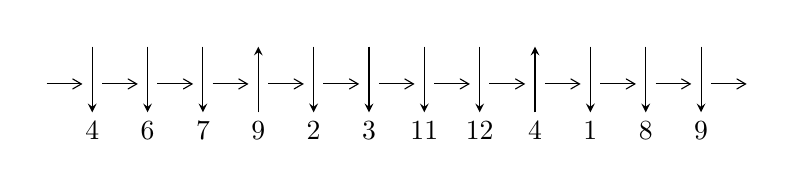
\begin{tikzpicture}[x=20pt, y=17pt]
	% nodes
	\node (C0) at (0, 0) {};
	\node (C1) at (1, 0) {};
	\node (C1U) at (1, +1) {};
	\node (C1D) at (1, -1) {4};

	\node (C2) at (2, 0) {};
	\node (C2U) at (2, +1) {};
	\node (C2D) at (2, -1) {6};

	\node (C3) at (3, 0) {};
	\node (C3U) at (3, +1) {};
	\node (C3D) at (3, -1) {7};

	\node (C4) at (4, 0) {};
	\node (C4U) at (4, +1) {};
	\node (C4D) at (4, -1) {9};

	\node (C5) at (5, 0) {};
	\node (C5U) at (5, +1) {};
	\node (C5D) at (5, -1) {2};

	\node (C6) at (6, 0) {};
	\node (C6U) at (6, +1) {};
	\node (C6D) at (6, -1) {3};

	\node (C7) at (7, 0) {};
	\node (C7U) at (7, +1) {};
	\node (C7D) at (7, -1) {11};

	\node (C8) at (8, 0) {};
	\node (C8U) at (8, +1) {};
	\node (C8D) at (8, -1) {12};

	\node (C9) at (9, 0) {};
	\node (C9U) at (9, +1) {};
	\node (C9D) at (9, -1) {4};

	\node (C10) at (10, 0) {};
	\node (C10U) at (10, +1) {};
	\node (C10D) at (10, -1) {1};

	\node (C11) at (11, 0) {};
	\node (C11U) at (11, +1) {};
	\node (C11D) at (11, -1) {8};

	\node (C12) at (12, 0) {};
	\node (C12U) at (12, +1) {};
	\node (C12D) at (12, -1) {9};
	\node (C13) at (13, 0) {};

	% arrows
	\draw[->,>={angle 60}]
	(C0) edge (C1) (C1) edge (C2) (C2) edge (C3) (C3) edge (C4) (C4) edge (C5) (C5) edge (C6) (C6) edge (C7) (C7) edge (C8) (C8) edge (C9) (C9) edge (C10) (C10) edge (C11) (C11) edge (C12) (C12) edge (C13) ;	\draw[->,>=stealth]
	(C1U) edge (C1D) (C2U) edge (C2D) (C3U) edge (C3D) (C4D) edge (C4U) (C5U) edge (C5D) (C6U) edge (C6D) (C7U) edge (C7D) (C8U) edge (C8D) (C9D) edge (C9U) (C10U) edge (C10D) (C11U) edge (C11D) (C12U) edge (C12D) ;
	\end{tikzpicture} \\
\hhline{~~} \\& 
\textbf{Solving Sequence} \\ \cline{2-2} 
 &
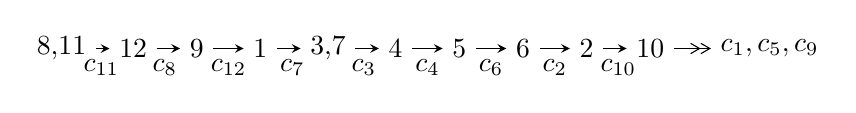
\begin{tikzpicture}[x=23pt, y=7pt]
	% node
	\node (A0) at (-1/8, 0) {8,11};
	\node (A1) at (1, 0) {12};
	\node (A2) at (2, 0) {9};
	\node (A3) at (3, 0) {1};
	\node (A4) at (65/16, 0) {3,7};
	\node (A5) at (41/8, 0) {4};
	\node (A6) at (49/8, 0) {5};
	\node (A7) at (57/8, 0) {6};
	\node (A8) at (65/8, 0) {2};
	\node (A9) at (73/8, 0) {10};
	\node (C1) at (1/2, -1) {$c_{11}$};
	\node (C2) at (3/2, -1) {$c_{8}$};
	\node (C3) at (5/2, -1) {$c_{12}$};
	\node (C4) at (7/2, -1) {$c_{7}$};
	\node (C5) at (37/8, -1) {$c_{3}$};
	\node (C6) at (45/8, -1) {$c_{4}$};
	\node (C7) at (53/8, -1) {$c_{6}$};
	\node (C8) at (61/8, -1) {$c_{2}$};
	\node (C9) at (69/8, -1) {$c_{10}$};
	\node (A10) at (11, 0) {$c_{1},c_{5},c_{9}$};

	% edge
	\draw[->,>=stealth]	
	(A0) edge (A1) (A1) edge (A2) (A2) edge (A3) (A3) edge (A4) (A4) edge (A5) (A5) edge (A6) (A6) edge (A7) (A7) edge (A8) (A8) edge (A9) ;
	\draw[->>,>={angle 60}]	
	(A9) edge (A10);
\end{tikzpicture} \\ 

\end{tabular} \\

\footnotetext{
The image of knot diagram is generated by the software ``\textbf{Draw programme}" developed by Andrew Bartholomew(\url{http://www.layer8.co.uk/maths/draw/index.htm\#Running-draw}), where we modified some parts for our purpose(\url{https://github.com/CATsTAILs/LinksPainter}).
}\phantom \\ \newline 
\centering \textbf{Ideals for irreducible components\footnotemark of $X_{\text{par}}$} 
 
\begin{align*}
I^u_{1}&=\langle 
- u^6+3 u^4- u^3- u^2+b+2 u+1,\;- u^6+3 u^4- u^3- u^2+a+2 u,\\
\phantom{I^u_{1}}&\phantom{= \langle  }u^9+u^8-5 u^7-4 u^6+8 u^5+3 u^4-5 u^3+2 u^2+3 u+1\rangle \\
I^u_{2}&=\langle 
4 u^{21}+3 u^{20}+\cdots+b-8 u,\;u^{21}-2 u^{20}+\cdots+a+6,\;u^{22}+2 u^{21}+\cdots-5 u+1\rangle \\
I^u_{3}&=\langle 
b-2 u-2,\;a-2 u-1,\;u^2- u-1\rangle \\
I^u_{4}&=\langle 
b+2,\;a+u,\;u^2- u-1\rangle \\
\\
\end{align*}
\raggedright * 4 irreducible components of $\dim_{\mathbb{C}}=0$, with total 35 representations.\\
\footnotetext{All coefficients of polynomials are rational numbers. But the coefficients are sometimes approximated in decimal forms when there is not enough margin.}
\newpage
\renewcommand{\arraystretch}{1}
\centering \section*{I. $I^u_{1}= \langle - u^6+3 u^4- u^3- u^2+b+2 u+1,\;- u^6+3 u^4- u^3- u^2+a+2 u,\;u^9+u^8+\cdots+3 u+1 \rangle$}
\flushleft \textbf{(i) Arc colorings}\\
\begin{tabular}{m{7pt} m{180pt} m{7pt} m{180pt} }
\flushright $a_{8}=$&$\begin{pmatrix}0\\u\end{pmatrix}$ \\
\flushright $a_{11}=$&$\begin{pmatrix}1\\0\end{pmatrix}$ \\
\flushright $a_{12}=$&$\begin{pmatrix}1\\u^2\end{pmatrix}$ \\
\flushright $a_{9}=$&$\begin{pmatrix}- u\\- u^3+u\end{pmatrix}$ \\
\flushright $a_{1}=$&$\begin{pmatrix}- u^2+1\\- u^4+2 u^2\end{pmatrix}$ \\
\flushright $a_{3}=$&$\begin{pmatrix}u^6-3 u^4+u^3+u^2-2 u\\u^6-3 u^4+u^3+u^2-2 u-1\end{pmatrix}$ \\
\flushright $a_{7}=$&$\begin{pmatrix}u\\u\end{pmatrix}$ \\
\flushright $a_{4}=$&$\begin{pmatrix}u^6-3 u^4+u^3+2 u^2-2 u\\u^6-3 u^4+u^3+2 u^2-2 u-1\end{pmatrix}$ \\
\flushright $a_{5}=$&$\begin{pmatrix}- u^8+5 u^6- u^5-7 u^4+4 u^3+2 u^2-4 u-1\\- u^8+5 u^6- u^5-7 u^4+3 u^3+2 u^2-2 u-1\end{pmatrix}$ \\
\flushright $a_{6}=$&$\begin{pmatrix}u^7-3 u^5+u^4+u^3-2 u^2+u\\u^7-3 u^5+u^4+u^3-2 u^2\end{pmatrix}$ \\
\flushright $a_{2}=$&$\begin{pmatrix}- u^8+4 u^6- u^5-4 u^4+3 u^3-2 u\\- u^8+4 u^6- u^5-4 u^4+3 u^3+u^2-2 u-1\end{pmatrix}$ \\
\flushright $a_{10}=$&$\begin{pmatrix}- u^6+3 u^4-2 u^2+1\\- u^8+4 u^6-4 u^4\end{pmatrix}$\\&\end{tabular}
\flushleft \textbf{(ii) Obstruction class $= -1$}\\~\\
\flushleft \textbf{(iii) Cusp Shapes $= -4 u^8-2 u^7+24 u^6+6 u^5-46 u^4+4 u^3+28 u^2-18 u-18$}\\~\\
\newpage\renewcommand{\arraystretch}{1}
\flushleft \textbf{(iv) u-Polynomials at the component}\newline \\
\begin{tabular}{m{50pt}|m{274pt}}
Crossings & \hspace{64pt}u-Polynomials at each crossing \\
\hline $$\begin{aligned}c_{1},c_{10}\end{aligned}$$&$\begin{aligned}
&u^9- u^8+7 u^7-2 u^6+16 u^5+3 u^4+9 u^3+10 u^2+3 u+1
\end{aligned}$\\
\hline $$\begin{aligned}c_{2},c_{3},c_{5}\\c_{6},c_{7},c_{8}\\c_{11},c_{12}\end{aligned}$$&$\begin{aligned}
&u^9+u^8-5 u^7-4 u^6+8 u^5+3 u^4-5 u^3+2 u^2+3 u+1
\end{aligned}$\\
\hline $$\begin{aligned}c_{4},c_{9}\end{aligned}$$&$\begin{aligned}
&u^9+5 u^8+10 u^7+9 u^6- u^5-15 u^4-22 u^3-16 u^2-8 u-4
\end{aligned}$\\
\hline
\end{tabular}\\~\\
\newpage\renewcommand{\arraystretch}{1}
\flushleft \textbf{(v) Riley Polynomials at the component}\newline \\
\begin{tabular}{m{50pt}|m{274pt}}
Crossings & \hspace{64pt}Riley Polynomials at each crossing \\
\hline $$\begin{aligned}c_{1},c_{10}\end{aligned}$$&$\begin{aligned}
&y^9+13 y^8+\cdots-11 y-1
\end{aligned}$\\
\hline $$\begin{aligned}c_{2},c_{3},c_{5}\\c_{6},c_{7},c_{8}\\c_{11},c_{12}\end{aligned}$$&$\begin{aligned}
&y^9-11 y^8+49 y^7-112 y^6+140 y^5-105 y^4+69 y^3-40 y^2+5 y-1
\end{aligned}$\\
\hline $$\begin{aligned}c_{4},c_{9}\end{aligned}$$&$\begin{aligned}
&y^9-5 y^8+8 y^7+5 y^6-25 y^5-13 y^4+92 y^3-24 y^2-64 y-16
\end{aligned}$\\
\hline
\end{tabular}\\~\\
\newpage\flushleft \textbf{(vi) Complex Volumes and Cusp Shapes}
$$\begin{array}{c|c|c}  
\text{Solutions to }I^u_{1}& \I (\text{vol} + \sqrt{-1}CS) & \text{Cusp shape}\\
 \hline 
\begin{aligned}
u &= \phantom{-}0.556651 + 0.655843 I \\
a &= -0.0328003 - 0.0846569 I \\
b &= -1.032800 - 0.084657 I\end{aligned}
 & \phantom{-}4.56735 - 4.47297 I & -7.81258 + 6.23831 I \\ \hline\begin{aligned}
u &= \phantom{-}0.556651 - 0.655843 I \\
a &= -0.0328003 + 0.0846569 I \\
b &= -1.032800 + 0.084657 I\end{aligned}
 & \phantom{-}4.56735 + 4.47297 I & -7.81258 - 6.23831 I \\ \hline\begin{aligned}
u &= -1.28665\phantom{ +0.000000I} \\
a &= -1.58604\phantom{ +0.000000I} \\
b &= -2.58604\phantom{ +0.000000I}\end{aligned}
 & -6.48693\phantom{ +0.000000I} & -13.7120\phantom{ +0.000000I} \\ \hline\begin{aligned}
u &= \phantom{-}1.51165 + 0.13243 I \\
a &= -1.75672 + 1.70564 I \\
b &= -2.75672 + 1.70564 I\end{aligned}
 & -13.17090 - 3.99995 I & -16.3846 + 2.3960 I \\ \hline\begin{aligned}
u &= \phantom{-}1.51165 - 0.13243 I \\
a &= -1.75672 - 1.70564 I \\
b &= -2.75672 - 1.70564 I\end{aligned}
 & -13.17090 + 3.99995 I & -16.3846 - 2.3960 I \\ \hline\begin{aligned}
u &= -0.338768 + 0.252040 I \\
a &= \phantom{-}0.829715 - 0.547946 I \\
b &= -0.170285 - 0.547946 I\end{aligned}
 & -0.531790 + 0.852880 I & -9.17076 - 8.14648 I \\ \hline\begin{aligned}
u &= -0.338768 - 0.252040 I \\
a &= \phantom{-}0.829715 + 0.547946 I \\
b &= -0.170285 + 0.547946 I\end{aligned}
 & -0.531790 - 0.852880 I & -9.17076 + 8.14648 I \\ \hline\begin{aligned}
u &= -1.58621 + 0.20573 I \\
a &= -3.24718 - 1.53651 I \\
b &= -4.24718 - 1.53651 I\end{aligned}
 & -9.8278 + 10.8008 I & -14.7759 - 5.3771 I \\ \hline\begin{aligned}
u &= -1.58621 - 0.20573 I \\
a &= -3.24718 + 1.53651 I \\
b &= -4.24718 + 1.53651 I\end{aligned}
 & -9.8278 - 10.8008 I & -14.7759 + 5.3771 I\\
 \hline 
 \end{array}$$\newpage\newpage\renewcommand{\arraystretch}{1}
\centering \section*{II. $I^u_{2}= \langle 4 u^{21}+3 u^{20}+\cdots+b-8 u,\;u^{21}-2 u^{20}+\cdots+a+6,\;u^{22}+2 u^{21}+\cdots-5 u+1 \rangle$}
\flushleft \textbf{(i) Arc colorings}\\
\begin{tabular}{m{7pt} m{180pt} m{7pt} m{180pt} }
\flushright $a_{8}=$&$\begin{pmatrix}0\\u\end{pmatrix}$ \\
\flushright $a_{11}=$&$\begin{pmatrix}1\\0\end{pmatrix}$ \\
\flushright $a_{12}=$&$\begin{pmatrix}1\\u^2\end{pmatrix}$ \\
\flushright $a_{9}=$&$\begin{pmatrix}- u\\- u^3+u\end{pmatrix}$ \\
\flushright $a_{1}=$&$\begin{pmatrix}- u^2+1\\- u^4+2 u^2\end{pmatrix}$ \\
\flushright $a_{3}=$&$\begin{pmatrix}- u^{21}+2 u^{20}+\cdots+13 u-6\\-4 u^{21}-3 u^{20}+\cdots-16 u^2+8 u\end{pmatrix}$ \\
\flushright $a_{7}=$&$\begin{pmatrix}u\\u\end{pmatrix}$ \\
\flushright $a_{4}=$&$\begin{pmatrix}2 u^{21}+4 u^{20}+\cdots+5 u-5\\- u^{21}- u^{20}+\cdots-8 u^2+1\end{pmatrix}$ \\
\flushright $a_{5}=$&$\begin{pmatrix}3 u^{20}+3 u^{19}+\cdots+15 u-7\\-3 u^{21}-3 u^{20}+\cdots-15 u^2+7 u\end{pmatrix}$ \\
\flushright $a_{6}=$&$\begin{pmatrix}- u^{21}+11 u^{19}+\cdots-17 u^3+9 u\\-2 u^{21}-2 u^{20}+\cdots-11 u^2+2 u\end{pmatrix}$ \\
\flushright $a_{2}=$&$\begin{pmatrix}- u^{20}- u^{19}+\cdots-7 u+1\\u^{21}+u^{20}+\cdots+6 u^3+8 u^2\end{pmatrix}$ \\
\flushright $a_{10}=$&$\begin{pmatrix}- u^6+3 u^4-2 u^2+1\\- u^8+4 u^6-4 u^4\end{pmatrix}$\\&\end{tabular}
\flushleft \textbf{(ii) Obstruction class $= -1$}\\~\\
\flushleft \textbf{(iii) Cusp Shapes $= 3 u^{20}+3 u^{19}-32 u^{18}-27 u^{17}+138 u^{16}+81 u^{15}-317 u^{14}-62 u^{13}+439 u^{12}-123 u^{11}-384 u^{10}+246 u^9+177 u^8-178 u^7-27 u^6+115 u^5+25 u^4-37 u^3+20 u^2+18 u-11$}\\~\\
\newpage\renewcommand{\arraystretch}{1}
\flushleft \textbf{(iv) u-Polynomials at the component}\newline \\
\begin{tabular}{m{50pt}|m{274pt}}
Crossings & \hspace{64pt}u-Polynomials at each crossing \\
\hline $$\begin{aligned}c_{1},c_{10}\end{aligned}$$&$\begin{aligned}
&u^{22}-4 u^{21}+\cdots-11 u-1
\end{aligned}$\\
\hline $$\begin{aligned}c_{2},c_{3},c_{5}\\c_{6},c_{7},c_{8}\\c_{11},c_{12}\end{aligned}$$&$\begin{aligned}
&u^{22}+2 u^{21}+\cdots-5 u+1
\end{aligned}$\\
\hline $$\begin{aligned}c_{4},c_{9}\end{aligned}$$&$\begin{aligned}
&(u^{11}-2 u^{10}-3 u^9+8 u^8-8 u^6+9 u^5-8 u^4-7 u^3+12 u^2+u-2)^2
\end{aligned}$\\
\hline
\end{tabular}\\~\\
\newpage\renewcommand{\arraystretch}{1}
\flushleft \textbf{(v) Riley Polynomials at the component}\newline \\
\begin{tabular}{m{50pt}|m{274pt}}
Crossings & \hspace{64pt}Riley Polynomials at each crossing \\
\hline $$\begin{aligned}c_{1},c_{10}\end{aligned}$$&$\begin{aligned}
&y^{22}+12 y^{21}+\cdots-103 y+1
\end{aligned}$\\
\hline $$\begin{aligned}c_{2},c_{3},c_{5}\\c_{6},c_{7},c_{8}\\c_{11},c_{12}\end{aligned}$$&$\begin{aligned}
&y^{22}-24 y^{21}+\cdots-27 y+1
\end{aligned}$\\
\hline $$\begin{aligned}c_{4},c_{9}\end{aligned}$$&$\begin{aligned}
&(y^{11}-10 y^{10}+\cdots+49 y-4)^{2}
\end{aligned}$\\
\hline
\end{tabular}\\~\\
\newpage\flushleft \textbf{(vi) Complex Volumes and Cusp Shapes}
$$\begin{array}{c|c|c}  
\text{Solutions to }I^u_{2}& \I (\text{vol} + \sqrt{-1}CS) & \text{Cusp shape}\\
 \hline 
\begin{aligned}
u &= \phantom{-}0.653871 + 0.639377 I \\
a &= \phantom{-}0.678912 + 0.802720 I \\
b &= \phantom{-}2.04567 - 0.21056 I\end{aligned}
 & -2.35449 - 7.64539 I & -11.71373 + 6.03391 I \\ \hline\begin{aligned}
u &= \phantom{-}0.653871 - 0.639377 I \\
a &= \phantom{-}0.678912 - 0.802720 I \\
b &= \phantom{-}2.04567 + 0.21056 I\end{aligned}
 & -2.35449 + 7.64539 I & -11.71373 - 6.03391 I \\ \hline\begin{aligned}
u &= \phantom{-}0.452757 + 0.672728 I \\
a &= -0.132038 - 0.926413 I \\
b &= \phantom{-}0.244470\phantom{ +0.000000I}\end{aligned}
 & \phantom{-}4.87434\phantom{ +0.000000I} & -6.59077 + 0. I\phantom{ +0.000000I} \\ \hline\begin{aligned}
u &= \phantom{-}0.452757 - 0.672728 I \\
a &= -0.132038 + 0.926413 I \\
b &= \phantom{-}0.244470\phantom{ +0.000000I}\end{aligned}
 & \phantom{-}4.87434\phantom{ +0.000000I} & -6.59077 + 0. I\phantom{ +0.000000I} \\ \hline\begin{aligned}
u &= \phantom{-}0.326778 + 0.705531 I \\
a &= -0.32042 + 2.18575 I \\
b &= \phantom{-}0.242416 + 0.347557 I\end{aligned}
 & -1.39120 + 3.13582 I & -9.76425 - 0.75545 I \\ \hline\begin{aligned}
u &= \phantom{-}0.326778 - 0.705531 I \\
a &= -0.32042 - 2.18575 I \\
b &= \phantom{-}0.242416 - 0.347557 I\end{aligned}
 & -1.39120 - 3.13582 I & -9.76425 + 0.75545 I \\ \hline\begin{aligned}
u &= -0.715155\phantom{ +0.000000I} \\
a &= \phantom{-}0.362929\phantom{ +0.000000I} \\
b &= \phantom{-}0.686958\phantom{ +0.000000I}\end{aligned}
 & -1.26486\phantom{ +0.000000I} & -6.07510\phantom{ +0.000000I} \\ \hline\begin{aligned}
u &= -1.300610 + 0.077299 I \\
a &= -1.58364 + 0.11845 I \\
b &= -2.57660\phantom{ +0.000000I}\end{aligned}
 & -6.48450\phantom{ +0.000000I} & -13.63121 + 0. I\phantom{ +0.000000I} \\ \hline\begin{aligned}
u &= -1.300610 - 0.077299 I \\
a &= -1.58364 - 0.11845 I \\
b &= -2.57660\phantom{ +0.000000I}\end{aligned}
 & -6.48450\phantom{ +0.000000I} & -13.63121 + 0. I\phantom{ +0.000000I} \\ \hline\begin{aligned}
u &= -0.472498 + 0.509885 I \\
a &= -0.670269 - 0.742959 I \\
b &= \phantom{-}0.829406 + 0.775983 I\end{aligned}
 & -6.60747 + 1.76997 I & -13.10604 - 3.70025 I\\
 \hline 
 \end{array}$$\newpage$$\begin{array}{c|c|c}  
\text{Solutions to }I^u_{2}& \I (\text{vol} + \sqrt{-1}CS) & \text{Cusp shape}\\
 \hline 
\begin{aligned}
u &= -0.472498 - 0.509885 I \\
a &= -0.670269 + 0.742959 I \\
b &= \phantom{-}0.829406 - 0.775983 I\end{aligned}
 & -6.60747 - 1.76997 I & -13.10604 + 3.70025 I \\ \hline\begin{aligned}
u &= \phantom{-}1.48308 + 0.04696 I \\
a &= \phantom{-}0.500256 - 1.109360 I \\
b &= \phantom{-}0.829406 - 0.775983 I\end{aligned}
 & -6.60747 - 1.76997 I & -13.10604 + 3.70025 I \\ \hline\begin{aligned}
u &= \phantom{-}1.48308 - 0.04696 I \\
a &= \phantom{-}0.500256 + 1.109360 I \\
b &= \phantom{-}0.829406 + 0.775983 I\end{aligned}
 & -6.60747 + 1.76997 I & -13.10604 - 3.70025 I \\ \hline\begin{aligned}
u &= -1.48082 + 0.20358 I \\
a &= \phantom{-}0.090121 - 0.149824 I \\
b &= \phantom{-}0.242416 + 0.347557 I\end{aligned}
 & -1.39120 + 3.13582 I & -9.76425 - 0.75545 I \\ \hline\begin{aligned}
u &= -1.48082 - 0.20358 I \\
a &= \phantom{-}0.090121 + 0.149824 I \\
b &= \phantom{-}0.242416 - 0.347557 I\end{aligned}
 & -1.39120 - 3.13582 I & -9.76425 + 0.75545 I \\ \hline\begin{aligned}
u &= -1.52066\phantom{ +0.000000I} \\
a &= \phantom{-}4.11109\phantom{ +0.000000I} \\
b &= \phantom{-}5.21838\phantom{ +0.000000I}\end{aligned}
 & -16.2219\phantom{ +0.000000I} & -13.6940\phantom{ +0.000000I} \\ \hline\begin{aligned}
u &= -1.54155 + 0.21133 I \\
a &= \phantom{-}1.57352 + 0.56059 I \\
b &= \phantom{-}2.04567 + 0.21056 I\end{aligned}
 & -2.35449 + 7.64539 I & -11.71373 - 6.03391 I \\ \hline\begin{aligned}
u &= -1.54155 - 0.21133 I \\
a &= \phantom{-}1.57352 - 0.56059 I \\
b &= \phantom{-}2.04567 - 0.21056 I\end{aligned}
 & -2.35449 - 7.64539 I & -11.71373 + 6.03391 I \\ \hline\begin{aligned}
u &= \phantom{-}0.443905\phantom{ +0.000000I} \\
a &= \phantom{-}1.87359\phantom{ +0.000000I} \\
b &= -1.80820\phantom{ +0.000000I}\end{aligned}
 & -9.54474\phantom{ +0.000000I} & \phantom{-}0.158940\phantom{ +0.000000I} \\ \hline\begin{aligned}
u &= \phantom{-}1.63437\phantom{ +0.000000I} \\
a &= -1.53660\phantom{ +0.000000I} \\
b &= -1.80820\phantom{ +0.000000I}\end{aligned}
 & -9.54474\phantom{ +0.000000I} & \phantom{-}0.158940\phantom{ +0.000000I}\\
 \hline 
 \end{array}$$\newpage$$\begin{array}{c|c|c}  
\text{Solutions to }I^u_{2}& \I (\text{vol} + \sqrt{-1}CS) & \text{Cusp shape}\\
 \hline 
\begin{aligned}
u &= \phantom{-}1.68381\phantom{ +0.000000I} \\
a &= \phantom{-}4.31528\phantom{ +0.000000I} \\
b &= \phantom{-}5.21838\phantom{ +0.000000I}\end{aligned}
 & -16.2219\phantom{ +0.000000I} & -13.6940\phantom{ +0.000000I} \\ \hline\begin{aligned}
u &= \phantom{-}0.231731\phantom{ +0.000000I} \\
a &= -2.39918\phantom{ +0.000000I} \\
b &= \phantom{-}0.686958\phantom{ +0.000000I}\end{aligned}
 & -1.26486\phantom{ +0.000000I} & -6.07510\phantom{ +0.000000I}\\
 \hline 
 \end{array}$$\newpage\newpage\renewcommand{\arraystretch}{1}
\centering \section*{III. $I^u_{3}= \langle b-2 u-2,\;a-2 u-1,\;u^2- u-1 \rangle$}
\flushleft \textbf{(i) Arc colorings}\\
\begin{tabular}{m{7pt} m{180pt} m{7pt} m{180pt} }
\flushright $a_{8}=$&$\begin{pmatrix}0\\u\end{pmatrix}$ \\
\flushright $a_{11}=$&$\begin{pmatrix}1\\0\end{pmatrix}$ \\
\flushright $a_{12}=$&$\begin{pmatrix}1\\u+1\end{pmatrix}$ \\
\flushright $a_{9}=$&$\begin{pmatrix}- u\\- u-1\end{pmatrix}$ \\
\flushright $a_{1}=$&$\begin{pmatrix}- u\\- u\end{pmatrix}$ \\
\flushright $a_{3}=$&$\begin{pmatrix}2 u+1\\2 u+2\end{pmatrix}$ \\
\flushright $a_{7}=$&$\begin{pmatrix}u\\u\end{pmatrix}$ \\
\flushright $a_{4}=$&$\begin{pmatrix}u\\u+1\end{pmatrix}$ \\
\flushright $a_{5}=$&$\begin{pmatrix}u\\u+1\end{pmatrix}$ \\
\flushright $a_{6}=$&$\begin{pmatrix}-2 u-2\\-3 u-2\end{pmatrix}$ \\
\flushright $a_{2}=$&$\begin{pmatrix}-2 u-1\\-3 u-1\end{pmatrix}$ \\
\flushright $a_{10}=$&$\begin{pmatrix}- u\\- u-1\end{pmatrix}$\\&\end{tabular}
\flushleft \textbf{(ii) Obstruction class $= 1$}\\~\\
\flushleft \textbf{(iii) Cusp Shapes $= -20$}\\~\\
\newpage\renewcommand{\arraystretch}{1}
\flushleft \textbf{(iv) u-Polynomials at the component}\newline \\
\begin{tabular}{m{50pt}|m{274pt}}
Crossings & \hspace{64pt}u-Polynomials at each crossing \\
\hline $$\begin{aligned}c_{1},c_{2},c_{3}\\c_{7},c_{8},c_{10}\end{aligned}$$&$\begin{aligned}
&u^2+u-1
\end{aligned}$\\
\hline $$\begin{aligned}c_{4},c_{9}\end{aligned}$$&$\begin{aligned}
&u^2
\end{aligned}$\\
\hline $$\begin{aligned}c_{5},c_{6},c_{11}\\c_{12}\end{aligned}$$&$\begin{aligned}
&u^2- u-1
\end{aligned}$\\
\hline
\end{tabular}\\~\\
\newpage\renewcommand{\arraystretch}{1}
\flushleft \textbf{(v) Riley Polynomials at the component}\newline \\
\begin{tabular}{m{50pt}|m{274pt}}
Crossings & \hspace{64pt}Riley Polynomials at each crossing \\
\hline $$\begin{aligned}c_{1},c_{2},c_{3}\\c_{5},c_{6},c_{7}\\c_{8},c_{10},c_{11}\\c_{12}\end{aligned}$$&$\begin{aligned}
&y^2-3 y+1
\end{aligned}$\\
\hline $$\begin{aligned}c_{4},c_{9}\end{aligned}$$&$\begin{aligned}
&y^2
\end{aligned}$\\
\hline
\end{tabular}\\~\\
\newpage\flushleft \textbf{(vi) Complex Volumes and Cusp Shapes}
$$\begin{array}{c|c|c}  
\text{Solutions to }I^u_{3}& \I (\text{vol} + \sqrt{-1}CS) & \text{Cusp shape}\\
 \hline 
\begin{aligned}
u &= -0.618034\phantom{ +0.000000I} \\
a &= -0.236068\phantom{ +0.000000I} \\
b &= \phantom{-}0.763932\phantom{ +0.000000I}\end{aligned}
 & -1.97392\phantom{ +0.000000I} & -20.0000\phantom{ +0.000000I} \\ \hline\begin{aligned}
u &= \phantom{-}1.61803\phantom{ +0.000000I} \\
a &= \phantom{-}4.23607\phantom{ +0.000000I} \\
b &= \phantom{-}5.23607\phantom{ +0.000000I}\end{aligned}
 & -17.7653\phantom{ +0.000000I} & -20.0000\phantom{ +0.000000I}\\
 \hline 
 \end{array}$$\newpage\newpage\renewcommand{\arraystretch}{1}
\centering \section*{IV. $I^u_{4}= \langle b+2,\;a+u,\;u^2- u-1 \rangle$}
\flushleft \textbf{(i) Arc colorings}\\
\begin{tabular}{m{7pt} m{180pt} m{7pt} m{180pt} }
\flushright $a_{8}=$&$\begin{pmatrix}0\\u\end{pmatrix}$ \\
\flushright $a_{11}=$&$\begin{pmatrix}1\\0\end{pmatrix}$ \\
\flushright $a_{12}=$&$\begin{pmatrix}1\\u+1\end{pmatrix}$ \\
\flushright $a_{9}=$&$\begin{pmatrix}- u\\- u-1\end{pmatrix}$ \\
\flushright $a_{1}=$&$\begin{pmatrix}- u\\- u\end{pmatrix}$ \\
\flushright $a_{3}=$&$\begin{pmatrix}- u\\-2\end{pmatrix}$ \\
\flushright $a_{7}=$&$\begin{pmatrix}u\\u\end{pmatrix}$ \\
\flushright $a_{4}=$&$\begin{pmatrix}- u+1\\-1\end{pmatrix}$ \\
\flushright $a_{5}=$&$\begin{pmatrix}- u+1\\-1\end{pmatrix}$ \\
\flushright $a_{6}=$&$\begin{pmatrix}u-1\\- u+2\end{pmatrix}$ \\
\flushright $a_{2}=$&$\begin{pmatrix}-2\\-2 u+1\end{pmatrix}$ \\
\flushright $a_{10}=$&$\begin{pmatrix}- u\\- u-1\end{pmatrix}$\\&\end{tabular}
\flushleft \textbf{(ii) Obstruction class $= 1$}\\~\\
\flushleft \textbf{(iii) Cusp Shapes $= -25$}\\~\\
\newpage\renewcommand{\arraystretch}{1}
\flushleft \textbf{(iv) u-Polynomials at the component}\newline \\
\begin{tabular}{m{50pt}|m{274pt}}
Crossings & \hspace{64pt}u-Polynomials at each crossing \\
\hline $$\begin{aligned}c_{1},c_{2},c_{3}\\c_{7},c_{8},c_{10}\end{aligned}$$&$\begin{aligned}
&u^2+u-1
\end{aligned}$\\
\hline $$\begin{aligned}c_{4},c_{9}\end{aligned}$$&$\begin{aligned}
&u^2
\end{aligned}$\\
\hline $$\begin{aligned}c_{5},c_{6},c_{11}\\c_{12}\end{aligned}$$&$\begin{aligned}
&u^2- u-1
\end{aligned}$\\
\hline
\end{tabular}\\~\\
\newpage\renewcommand{\arraystretch}{1}
\flushleft \textbf{(v) Riley Polynomials at the component}\newline \\
\begin{tabular}{m{50pt}|m{274pt}}
Crossings & \hspace{64pt}Riley Polynomials at each crossing \\
\hline $$\begin{aligned}c_{1},c_{2},c_{3}\\c_{5},c_{6},c_{7}\\c_{8},c_{10},c_{11}\\c_{12}\end{aligned}$$&$\begin{aligned}
&y^2-3 y+1
\end{aligned}$\\
\hline $$\begin{aligned}c_{4},c_{9}\end{aligned}$$&$\begin{aligned}
&y^2
\end{aligned}$\\
\hline
\end{tabular}\\~\\
\newpage\flushleft \textbf{(vi) Complex Volumes and Cusp Shapes}
$$\begin{array}{c|c|c}  
\text{Solutions to }I^u_{4}& \I (\text{vol} + \sqrt{-1}CS) & \text{Cusp shape}\\
 \hline 
\begin{aligned}
u &= -0.618034\phantom{ +0.000000I} \\
a &= \phantom{-}0.618034\phantom{ +0.000000I} \\
b &= -2.00000\phantom{ +0.000000I}\end{aligned}
 & -9.86960\phantom{ +0.000000I} & -25.0000\phantom{ +0.000000I} \\ \hline\begin{aligned}
u &= \phantom{-}1.61803\phantom{ +0.000000I} \\
a &= -1.61803\phantom{ +0.000000I} \\
b &= -2.00000\phantom{ +0.000000I}\end{aligned}
 & -9.86960\phantom{ +0.000000I} & -25.0000\phantom{ +0.000000I}\\
 \hline 
 \end{array}$$\newpage
\newpage\renewcommand{\arraystretch}{1}
\centering \section*{ V. u-Polynomials}
\begin{tabular}{m{50pt}|m{274pt}}
Crossings & \hspace{64pt}u-Polynomials at each crossing \\
\hline $$\begin{aligned}c_{1},c_{10}\end{aligned}$$&$\begin{aligned}
&((u^2+u-1)^2)(u^9- u^8+\cdots+3 u+1)\\
&\cdot(u^{22}-4 u^{21}+\cdots-11 u-1)
\end{aligned}$\\
\hline $$\begin{aligned}c_{2},c_{3},c_{7}\\c_{8}\end{aligned}$$&$\begin{aligned}
&(u^2+u-1)^2(u^9+u^8-5 u^7-4 u^6+8 u^5+3 u^4-5 u^3+2 u^2+3 u+1)\\
&\cdot(u^{22}+2 u^{21}+\cdots-5 u+1)
\end{aligned}$\\
\hline $$\begin{aligned}c_{4},c_{9}\end{aligned}$$&$\begin{aligned}
&u^4(u^9+5 u^8+10 u^7+9 u^6- u^5-15 u^4-22 u^3-16 u^2-8 u-4)\\
&\cdot(u^{11}-2 u^{10}-3 u^9+8 u^8-8 u^6+9 u^5-8 u^4-7 u^3+12 u^2+u-2)^2
\end{aligned}$\\
\hline $$\begin{aligned}c_{5},c_{6},c_{11}\\c_{12}\end{aligned}$$&$\begin{aligned}
&(u^2- u-1)^2(u^9+u^8-5 u^7-4 u^6+8 u^5+3 u^4-5 u^3+2 u^2+3 u+1)\\
&\cdot(u^{22}+2 u^{21}+\cdots-5 u+1)
\end{aligned}$\\
\hline
\end{tabular}\newpage\renewcommand{\arraystretch}{1}
\centering \section*{ VI. Riley Polynomials}
\begin{tabular}{m{50pt}|m{274pt}}
Crossings & \hspace{64pt}Riley Polynomials at each crossing \\
\hline $$\begin{aligned}c_{1},c_{10}\end{aligned}$$&$\begin{aligned}
&((y^2-3 y+1)^2)(y^9+13 y^8+\cdots-11 y-1)\\
&\cdot(y^{22}+12 y^{21}+\cdots-103 y+1)
\end{aligned}$\\
\hline $$\begin{aligned}c_{2},c_{3},c_{5}\\c_{6},c_{7},c_{8}\\c_{11},c_{12}\end{aligned}$$&$\begin{aligned}
&(y^2-3 y+1)^2\\
&\cdot(y^9-11 y^8+49 y^7-112 y^6+140 y^5-105 y^4+69 y^3-40 y^2+5 y-1)\\
&\cdot(y^{22}-24 y^{21}+\cdots-27 y+1)
\end{aligned}$\\
\hline $$\begin{aligned}c_{4},c_{9}\end{aligned}$$&$\begin{aligned}
&y^4(y^9-5 y^8+8 y^7+5 y^6-25 y^5-13 y^4+92 y^3-24 y^2-64 y-16)\\
&\cdot(y^{11}-10 y^{10}+\cdots+49 y-4)^{2}
\end{aligned}$\\
\hline
\end{tabular}
\vskip 2pc
\end{document}